\documentclass{standalone}

\usepackage{tikz}
\usepackage{amsfonts}
\usetikzlibrary{positioning, mindmap, shadows, shapes}

\begin{document}
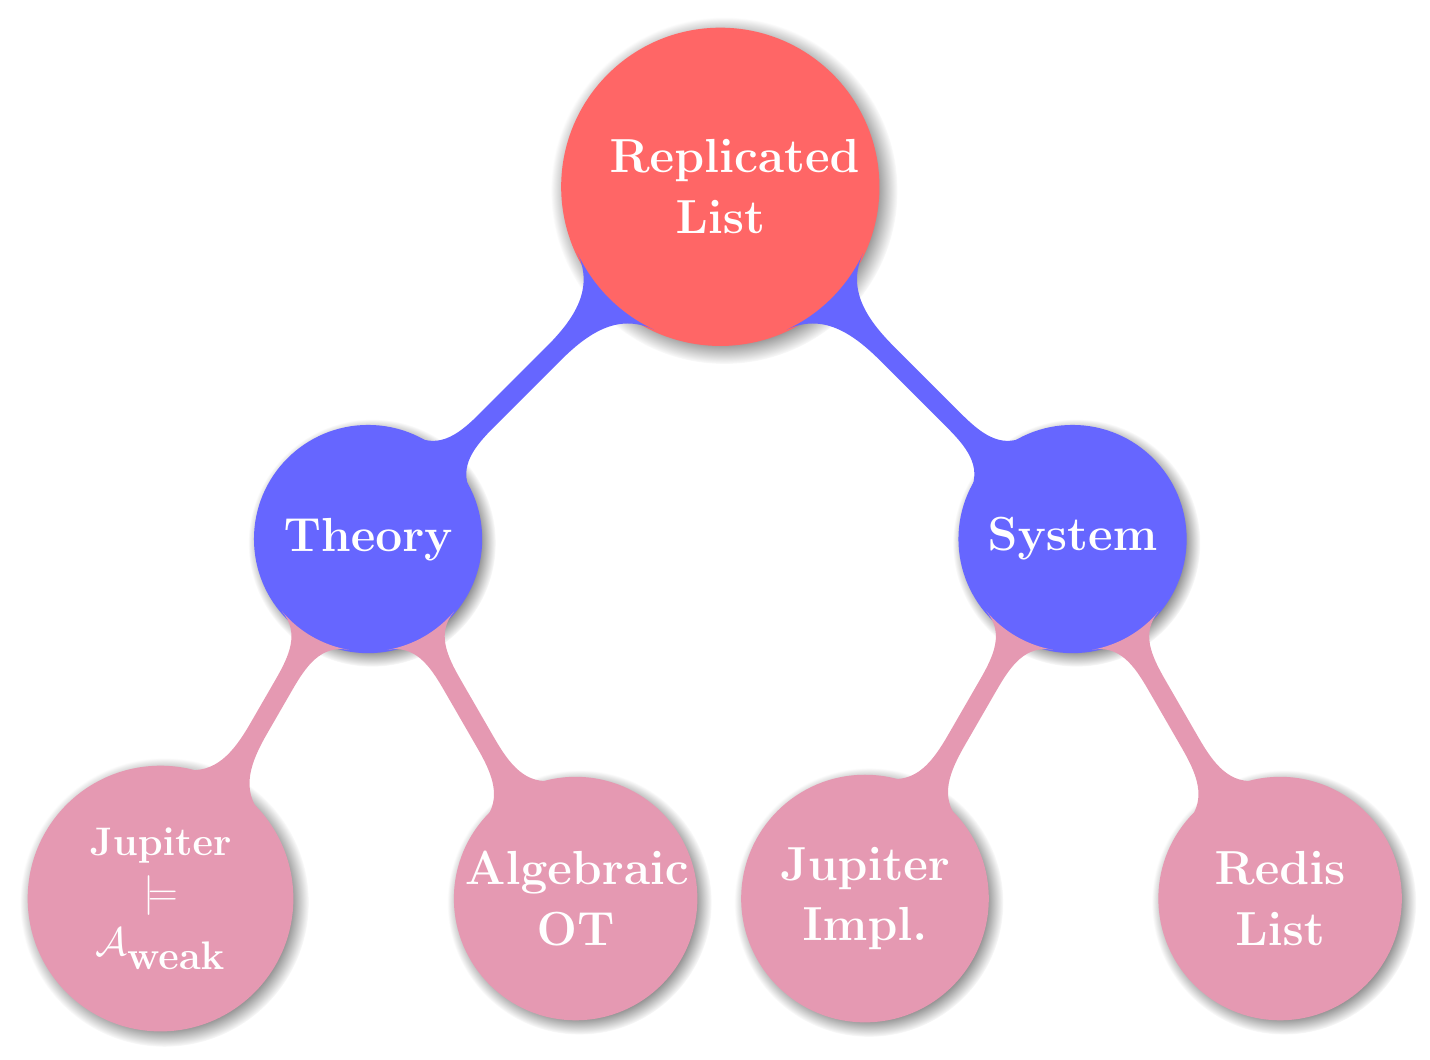
\begin{tikzpicture}

\path[mindmap,
    text = white,
    every node/.style = {
      concept,
      circular drop shadow
    },
    root/.style = {
      concept color = red!60,
      font = \LARGE\bfseries, 
      text width = 8em
    },
    level 1 concept/.append style = {
      concept color = blue!60,
      font = \LARGE\bfseries,
      sibling angle = 90,
      text width = 8em,
      level distance = 18em,
      inner sep = 0pt
    },
    level 2 concept/.append style = {
      concept color = purple!40,
      font = \LARGE\bfseries,
      align = center,
      sibling angle = 60,
      text width = 8em,
      level distance = 15em
    },
  ]
  node [root] {Replicated \\ List} [counterclockwise from = 225]
    child [] {
      node {Theory} [counterclockwise from = 240]
	child [] {node (cjupiter) [font = \Large\bfseries] {$\textrm{Jupiter}$ \\ $\models$ \\ $\mathcal{A}_{\textrm{weak}}$}}
	child [] {node (aot) [] {Algebraic \\ OT}}
    }
    child [] {
      node {System} [counterclockwise from = 240]
	child [] {node (jupiter) [] {Jupiter \\ Impl.}}
	child [] {node (rlist) [] {Redis \\ List}}
    };
\end{tikzpicture}
\end{document}